\documentclass[11pt,a4paper,oneside]{article}
\usepackage{amsmath,amsthm,amsfonts,amssymb}
\usepackage{pst-eucl,pstricks,pstricks-add,multido, pst-plot}
\usepackage[utf8]{inputenc}
%\usepackage[latin1]{inputenc}
\usepackage[spanish,activeacute]{babel}
\usepackage[a4paper,margin=2.5cm]{geometry}
\usepackage{times}
\usepackage[T1]{fontenc}
\usepackage{titlesec}
\usepackage{url}
\usepackage{float}
\usepackage{cite}
\usepackage{graphicx}
\usepackage{wrapfig}
\usepackage{lipsum}
\usepackage{multicol}
\usepackage{float}
\usepackage{lmodern}
\usepackage{epstopdf}
\parindent=0mm
\usepackage{color, colortbl}
\definecolor{azul}{rgb}{0.63, 0.79, 0.95}

\newcommand*{\titleBOOK}{\begingroup
%\raggedleft
\centering
\vspace*{\baselineskip}
\vspace*{\baselineskip}
{\Huge\scshape Lecture Notes}\\[10mm]
%{\Large \includegraphics[scale=0.25]{uah.pdf}}\\[35mm]
{\Huge\scshape Non Life  \\[5mm]
Insurance} \\ [\baselineskip]
{\Large\bfseries First Draft}\\[0.3 \textheight]
{\Large Prof. Dr. Ricardo Gatto}\\
%{\large\scshape MS-PLUS, Inc.}\par
\vfill
\begin{center}
{\scshape Switzerland-Spain-Ecuador}\\
\rule{\textwidth}{0.5pt}
\end{center}
\vspace*{\baselineskip}
\endgroup}



\usepackage{Sweave}
\begin{document}
\Sconcordance{concordance:MatematicaNoVida.tex:MatematicaNoVida.Rnw:%
1 47 1 1 0 21 1 1 10 1 2 126 1 1 7 1 2 46 1}

\titleBOOK
\newpage

\tableofcontents
\newpage


\section{Individual Risk and Distributions}
A non negative random variable is called a \textbf{loss} and it its distribution a \textbf{loss distribution}.\\
$X\sim Exponential(\alpha)$ means that $X$ has density $f_X(x)=\alpha e^{-\alpha x}$ and distribution function (d.f) $F_X(x)=1-e^{-\alpha x}$ $\forall x>0$ and $\alpha>0$.\\


Let $Y=e^x$, 
\begin{align*}
F_Y(Y) &= F_X(log Y)\\
&=1-e^{\alpha log (y)}\\
&=1-y^{-\alpha}
\end{align*}
Is called the \textbf{Pareto Distribution}. If $Y$ follows a Pareto distribution, denoted  $Y\sim Pareto(\alpha)$

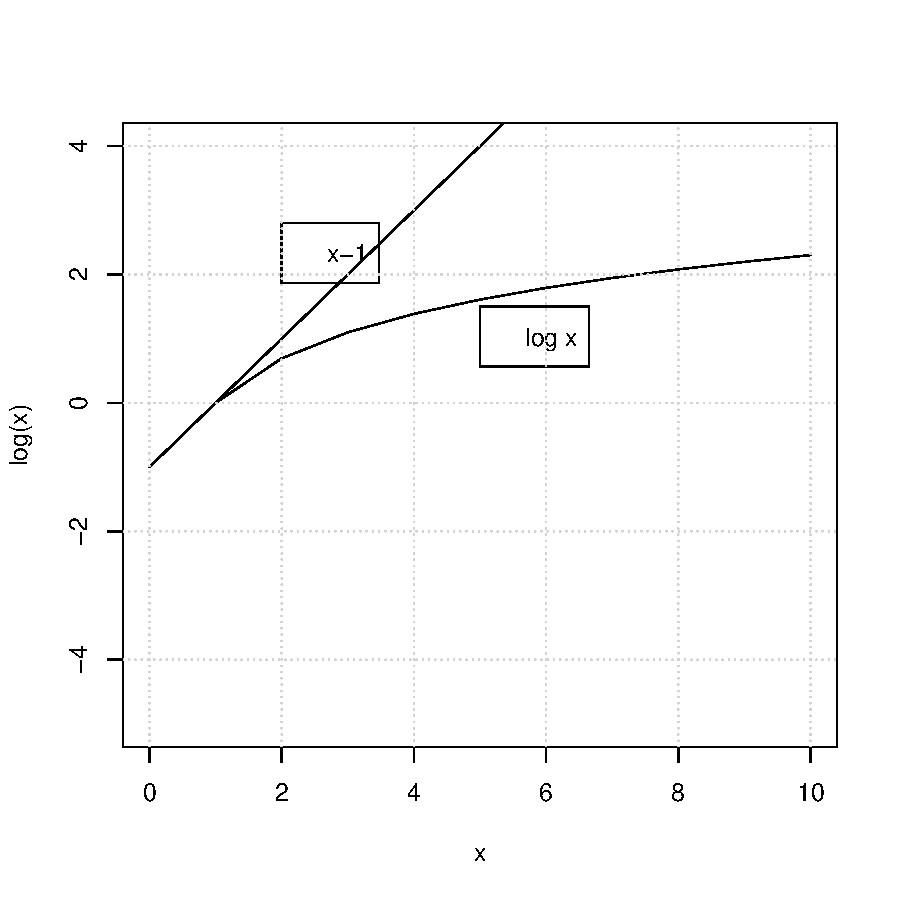
\includegraphics{MatematicaNoVida-examplePlot}

$X\sim Exponential (\lambda)$ and $Y\sim X^{\frac{1}{\tau}}$ $\forall \tau>0$
\begin{align*}
F_Y(Y) &= F_X(Y^{\tau})\\
&=1-e^{-\lambda y^{\tau}} \ \ \ \ \forall y>0\\
\end{align*}
$Y$ follows the \textbf{Weibull distribution}, $\tau$ is called the Weibull index.\\ It is denoted by $Y\sim Weibull(\tau,\lambda)$


\section{Thursday 09/03/17}

\subsection{Distribution of the largest claim amount}

The distribution of the largest loss is very important in \textbf{risk management}.

We will derive asymptotic aproximation of standardized maxima.

Let $X_1,...,X_n$ be independent losses with distribution function (d.f) $F$ and define $$M_n=max\{X_1,...,X_n\}$$


\begin{align*}
P[M_n\leq n] &=P[X_1\leqx,..,X_n\leq x]\\
&=F^n(x) \ \ \forall x>0\\
\end{align*}

Let $\bar{x}=sup\{x>0|F(x)<1\}$.

Assume $E[M_n]<\infty$, then $E[M_n]=\displaystyle\int_{0}^{\bar{x}}\{1-F^n(x)\}dx\xrightarrow{n\rightarrow \infty}{\bar{x}}$.

Assume $E[M^2_n]<\infty$, then $E[M_n^2]=\displaystyle\int_{0}^{\bar{x}}x\{1-F^n(x)\}dx\xrightarrow{n\rightarrow \infty}{\bar{x}^2}$

$Var(M_n)=E[M^2_n]-E^2[M_n]\xrightarrow{n\rightarrow \infty}{\bar{x}^2-\bar{x}^2}=0$, assuming $\bar{x}=0$.

Thus the asymptotic distribution of $M_n$ is degenerate (the total mass is over $\bar{x}$). SO if we want to compute this asymptotic distribution, we must consider the standardization $\frac{M_n-b_n}{a_n}$.

Before studying these asymptotic approximation we give some examples with finite sample.
\subsection{Examples}
The distribution  of the monthly largest loss is Gumbel $F(x)=G(\frac{x-\mu}{\sigma})$ where $G(x)=exp\{-e^{-x}\}\ \ x\in\mathbb{R}$, what is the distribution of the annual maximum?
\begin{align*}
F^12&=exp\{-12e^{-\frac{x-\mu}{\sigma}}\}\\
&=exp\{-e^{-\frac{x-\mu}{\sigma}+log 12}\}\\
&=exp\{-e^{-\frac{x-(\mu+\sigma log 12)}{\sigma}}\}
\end{align*}
It is thus agian GUmbel, with another location parameter with Frechet monthly largest loss, viz. with $G(x)=exp\{-x^{-\alpha}\}\ \ x>0$, we have $F^{12}(x)=exp\{-12\(\frac{x-\mu}{\sigma}\)^{-\alpha}\}=exp\{-(\frac{x-\mu}{12^{\frac{1}{\alpha}}\sigma})^{-\alpha}\}$
It is again Fréchet with another scale parameter. Because of this algebraic closure property, the Gumbel and the Frechet distributions are called max-stable.
We consider the slight generalization where the sample size is the random variable $N$.

Let $M_N=max\{X_1,...,X_N\}$. Assume $N$ independent of $X_1,X_2,....$
\begin{align*}
P[M_N\leq x]&=\displaystyle\sum_{n=0}^{\infty}P[M_N\leq x|N=n]P[N=n]\\
&=\displaystyle\sum_{n=0}^{\infty}F^n(x)P[N=n]\\
&=G_N(F(x))\ \ \ \forall x\geq 0\\
\end{align*}
Where $M_0=0$ and $G_N(v)=\displaystyle\sum_{n=0}^{\infty}v^nP[N=n]$ is the generating function of $N$.

Thus $P[M_N\leq 0]$ if $F(0)=0$
\end{document}
